% Options for packages loaded elsewhere
\PassOptionsToPackage{unicode}{hyperref}
\PassOptionsToPackage{hyphens}{url}
\PassOptionsToPackage{dvipsnames,svgnames,x11names}{xcolor}
%
\documentclass[
  letterpaper,
  DIV=11,
  numbers=noendperiod]{scrreprt}

\usepackage{amsmath,amssymb}
\usepackage{lmodern}
\usepackage{iftex}
\ifPDFTeX
  \usepackage[T1]{fontenc}
  \usepackage[utf8]{inputenc}
  \usepackage{textcomp} % provide euro and other symbols
\else % if luatex or xetex
  \usepackage{unicode-math}
  \defaultfontfeatures{Scale=MatchLowercase}
  \defaultfontfeatures[\rmfamily]{Ligatures=TeX,Scale=1}
\fi
% Use upquote if available, for straight quotes in verbatim environments
\IfFileExists{upquote.sty}{\usepackage{upquote}}{}
\IfFileExists{microtype.sty}{% use microtype if available
  \usepackage[]{microtype}
  \UseMicrotypeSet[protrusion]{basicmath} % disable protrusion for tt fonts
}{}
\makeatletter
\@ifundefined{KOMAClassName}{% if non-KOMA class
  \IfFileExists{parskip.sty}{%
    \usepackage{parskip}
  }{% else
    \setlength{\parindent}{0pt}
    \setlength{\parskip}{6pt plus 2pt minus 1pt}}
}{% if KOMA class
  \KOMAoptions{parskip=half}}
\makeatother
\usepackage{xcolor}
\setlength{\emergencystretch}{3em} % prevent overfull lines
\setcounter{secnumdepth}{5}
% Make \paragraph and \subparagraph free-standing
\ifx\paragraph\undefined\else
  \let\oldparagraph\paragraph
  \renewcommand{\paragraph}[1]{\oldparagraph{#1}\mbox{}}
\fi
\ifx\subparagraph\undefined\else
  \let\oldsubparagraph\subparagraph
  \renewcommand{\subparagraph}[1]{\oldsubparagraph{#1}\mbox{}}
\fi

\usepackage{color}
\usepackage{fancyvrb}
\newcommand{\VerbBar}{|}
\newcommand{\VERB}{\Verb[commandchars=\\\{\}]}
\DefineVerbatimEnvironment{Highlighting}{Verbatim}{commandchars=\\\{\}}
% Add ',fontsize=\small' for more characters per line
\usepackage{framed}
\definecolor{shadecolor}{RGB}{241,243,245}
\newenvironment{Shaded}{\begin{snugshade}}{\end{snugshade}}
\newcommand{\AlertTok}[1]{\textcolor[rgb]{0.68,0.00,0.00}{#1}}
\newcommand{\AnnotationTok}[1]{\textcolor[rgb]{0.37,0.37,0.37}{#1}}
\newcommand{\AttributeTok}[1]{\textcolor[rgb]{0.40,0.45,0.13}{#1}}
\newcommand{\BaseNTok}[1]{\textcolor[rgb]{0.68,0.00,0.00}{#1}}
\newcommand{\BuiltInTok}[1]{\textcolor[rgb]{0.00,0.23,0.31}{#1}}
\newcommand{\CharTok}[1]{\textcolor[rgb]{0.13,0.47,0.30}{#1}}
\newcommand{\CommentTok}[1]{\textcolor[rgb]{0.37,0.37,0.37}{#1}}
\newcommand{\CommentVarTok}[1]{\textcolor[rgb]{0.37,0.37,0.37}{\textit{#1}}}
\newcommand{\ConstantTok}[1]{\textcolor[rgb]{0.56,0.35,0.01}{#1}}
\newcommand{\ControlFlowTok}[1]{\textcolor[rgb]{0.00,0.23,0.31}{#1}}
\newcommand{\DataTypeTok}[1]{\textcolor[rgb]{0.68,0.00,0.00}{#1}}
\newcommand{\DecValTok}[1]{\textcolor[rgb]{0.68,0.00,0.00}{#1}}
\newcommand{\DocumentationTok}[1]{\textcolor[rgb]{0.37,0.37,0.37}{\textit{#1}}}
\newcommand{\ErrorTok}[1]{\textcolor[rgb]{0.68,0.00,0.00}{#1}}
\newcommand{\ExtensionTok}[1]{\textcolor[rgb]{0.00,0.23,0.31}{#1}}
\newcommand{\FloatTok}[1]{\textcolor[rgb]{0.68,0.00,0.00}{#1}}
\newcommand{\FunctionTok}[1]{\textcolor[rgb]{0.28,0.35,0.67}{#1}}
\newcommand{\ImportTok}[1]{\textcolor[rgb]{0.00,0.46,0.62}{#1}}
\newcommand{\InformationTok}[1]{\textcolor[rgb]{0.37,0.37,0.37}{#1}}
\newcommand{\KeywordTok}[1]{\textcolor[rgb]{0.00,0.23,0.31}{#1}}
\newcommand{\NormalTok}[1]{\textcolor[rgb]{0.00,0.23,0.31}{#1}}
\newcommand{\OperatorTok}[1]{\textcolor[rgb]{0.37,0.37,0.37}{#1}}
\newcommand{\OtherTok}[1]{\textcolor[rgb]{0.00,0.23,0.31}{#1}}
\newcommand{\PreprocessorTok}[1]{\textcolor[rgb]{0.68,0.00,0.00}{#1}}
\newcommand{\RegionMarkerTok}[1]{\textcolor[rgb]{0.00,0.23,0.31}{#1}}
\newcommand{\SpecialCharTok}[1]{\textcolor[rgb]{0.37,0.37,0.37}{#1}}
\newcommand{\SpecialStringTok}[1]{\textcolor[rgb]{0.13,0.47,0.30}{#1}}
\newcommand{\StringTok}[1]{\textcolor[rgb]{0.13,0.47,0.30}{#1}}
\newcommand{\VariableTok}[1]{\textcolor[rgb]{0.07,0.07,0.07}{#1}}
\newcommand{\VerbatimStringTok}[1]{\textcolor[rgb]{0.13,0.47,0.30}{#1}}
\newcommand{\WarningTok}[1]{\textcolor[rgb]{0.37,0.37,0.37}{\textit{#1}}}

\providecommand{\tightlist}{%
  \setlength{\itemsep}{0pt}\setlength{\parskip}{0pt}}\usepackage{longtable,booktabs,array}
\usepackage{calc} % for calculating minipage widths
% Correct order of tables after \paragraph or \subparagraph
\usepackage{etoolbox}
\makeatletter
\patchcmd\longtable{\par}{\if@noskipsec\mbox{}\fi\par}{}{}
\makeatother
% Allow footnotes in longtable head/foot
\IfFileExists{footnotehyper.sty}{\usepackage{footnotehyper}}{\usepackage{footnote}}
\makesavenoteenv{longtable}
\usepackage{graphicx}
\makeatletter
\def\maxwidth{\ifdim\Gin@nat@width>\linewidth\linewidth\else\Gin@nat@width\fi}
\def\maxheight{\ifdim\Gin@nat@height>\textheight\textheight\else\Gin@nat@height\fi}
\makeatother
% Scale images if necessary, so that they will not overflow the page
% margins by default, and it is still possible to overwrite the defaults
% using explicit options in \includegraphics[width, height, ...]{}
\setkeys{Gin}{width=\maxwidth,height=\maxheight,keepaspectratio}
% Set default figure placement to htbp
\makeatletter
\def\fps@figure{htbp}
\makeatother
\newlength{\cslhangindent}
\setlength{\cslhangindent}{1.5em}
\newlength{\csllabelwidth}
\setlength{\csllabelwidth}{3em}
\newlength{\cslentryspacingunit} % times entry-spacing
\setlength{\cslentryspacingunit}{\parskip}
\newenvironment{CSLReferences}[2] % #1 hanging-ident, #2 entry spacing
 {% don't indent paragraphs
  \setlength{\parindent}{0pt}
  % turn on hanging indent if param 1 is 1
  \ifodd #1
  \let\oldpar\par
  \def\par{\hangindent=\cslhangindent\oldpar}
  \fi
  % set entry spacing
  \setlength{\parskip}{#2\cslentryspacingunit}
 }%
 {}
\usepackage{calc}
\newcommand{\CSLBlock}[1]{#1\hfill\break}
\newcommand{\CSLLeftMargin}[1]{\parbox[t]{\csllabelwidth}{#1}}
\newcommand{\CSLRightInline}[1]{\parbox[t]{\linewidth - \csllabelwidth}{#1}\break}
\newcommand{\CSLIndent}[1]{\hspace{\cslhangindent}#1}

\KOMAoption{captions}{tableheading}
\makeatletter
\makeatother
\makeatletter
\@ifpackageloaded{bookmark}{}{\usepackage{bookmark}}
\makeatother
\makeatletter
\@ifpackageloaded{caption}{}{\usepackage{caption}}
\AtBeginDocument{%
\ifdefined\contentsname
  \renewcommand*\contentsname{Table of contents}
\else
  \newcommand\contentsname{Table of contents}
\fi
\ifdefined\listfigurename
  \renewcommand*\listfigurename{List of Figures}
\else
  \newcommand\listfigurename{List of Figures}
\fi
\ifdefined\listtablename
  \renewcommand*\listtablename{List of Tables}
\else
  \newcommand\listtablename{List of Tables}
\fi
\ifdefined\figurename
  \renewcommand*\figurename{Figure}
\else
  \newcommand\figurename{Figure}
\fi
\ifdefined\tablename
  \renewcommand*\tablename{Table}
\else
  \newcommand\tablename{Table}
\fi
}
\@ifpackageloaded{float}{}{\usepackage{float}}
\floatstyle{ruled}
\@ifundefined{c@chapter}{\newfloat{codelisting}{h}{lop}}{\newfloat{codelisting}{h}{lop}[chapter]}
\floatname{codelisting}{Listing}
\newcommand*\listoflistings{\listof{codelisting}{List of Listings}}
\makeatother
\makeatletter
\@ifpackageloaded{caption}{}{\usepackage{caption}}
\@ifpackageloaded{subcaption}{}{\usepackage{subcaption}}
\makeatother
\makeatletter
\@ifpackageloaded{tcolorbox}{}{\usepackage[many]{tcolorbox}}
\makeatother
\makeatletter
\@ifundefined{shadecolor}{\definecolor{shadecolor}{rgb}{.97, .97, .97}}
\makeatother
\makeatletter
\makeatother
\ifLuaTeX
  \usepackage{selnolig}  % disable illegal ligatures
\fi
\IfFileExists{bookmark.sty}{\usepackage{bookmark}}{\usepackage{hyperref}}
\IfFileExists{xurl.sty}{\usepackage{xurl}}{} % add URL line breaks if available
\urlstyle{same} % disable monospaced font for URLs
\hypersetup{
  pdftitle={Computational Publishing for Archives},
  pdfauthor={Simon Worthington},
  colorlinks=true,
  linkcolor={blue},
  filecolor={Maroon},
  citecolor={Blue},
  urlcolor={Blue},
  pdfcreator={LaTeX via pandoc}}

\title{Computational Publishing for Archives}
\author{Simon Worthington}
\date{9/11/22}

\begin{document}
\maketitle
\ifdefined\Shaded\renewenvironment{Shaded}{\begin{tcolorbox}[interior hidden, borderline west={3pt}{0pt}{shadecolor}, sharp corners, boxrule=0pt, frame hidden, breakable, enhanced]}{\end{tcolorbox}}\fi

\renewcommand*\contentsname{Table of contents}
{
\hypersetup{linkcolor=}
\setcounter{tocdepth}{2}
\tableofcontents
}
\bookmarksetup{startatroot}

\hypertarget{preface}{%
\chapter*{Preface}\label{preface}}
\addcontentsline{toc}{chapter}{Preface}

\markboth{Preface}{Preface}

This is a Quarto book.

To learn more about Quarto books visit
\url{https://quarto.org/docs/books}.

\bookmarksetup{startatroot}

\hypertarget{introduction}{%
\chapter{Introduction}\label{introduction}}

This is a book created from markdown and executable code.

See Knuth (1984) for additional discussion of literate programming.

\bookmarksetup{startatroot}

\hypertarget{summary}{%
\chapter{Summary}\label{summary}}

In summary, this book has no content whatsoever.

\bookmarksetup{startatroot}

\hypertarget{quarto-basics}{%
\chapter{Quarto Basics}\label{quarto-basics}}

For a demonstration of a line plot on a polar axis, see
Figure~\ref{fig-polar}.

\begin{Shaded}
\begin{Highlighting}[]
\ImportTok{import}\NormalTok{ numpy }\ImportTok{as}\NormalTok{ np}
\ImportTok{import}\NormalTok{ matplotlib.pyplot }\ImportTok{as}\NormalTok{ plt}

\NormalTok{r }\OperatorTok{=}\NormalTok{ np.arange(}\DecValTok{0}\NormalTok{, }\DecValTok{2}\NormalTok{, }\FloatTok{0.01}\NormalTok{)}
\NormalTok{theta }\OperatorTok{=} \DecValTok{2} \OperatorTok{*}\NormalTok{ np.pi }\OperatorTok{*}\NormalTok{ r}
\NormalTok{fig, ax }\OperatorTok{=}\NormalTok{ plt.subplots(}
\NormalTok{  subplot\_kw }\OperatorTok{=}\NormalTok{ \{}\StringTok{\textquotesingle{}projection\textquotesingle{}}\NormalTok{: }\StringTok{\textquotesingle{}polar\textquotesingle{}}\NormalTok{\}}
\NormalTok{)}
\NormalTok{ax.plot(theta, r)}
\NormalTok{ax.set\_rticks([}\FloatTok{0.5}\NormalTok{, }\DecValTok{1}\NormalTok{, }\FloatTok{1.5}\NormalTok{, }\DecValTok{2}\NormalTok{])}
\NormalTok{ax.grid(}\VariableTok{True}\NormalTok{)}
\NormalTok{plt.show()}
\end{Highlighting}
\end{Shaded}

\begin{figure}[H]

{\centering 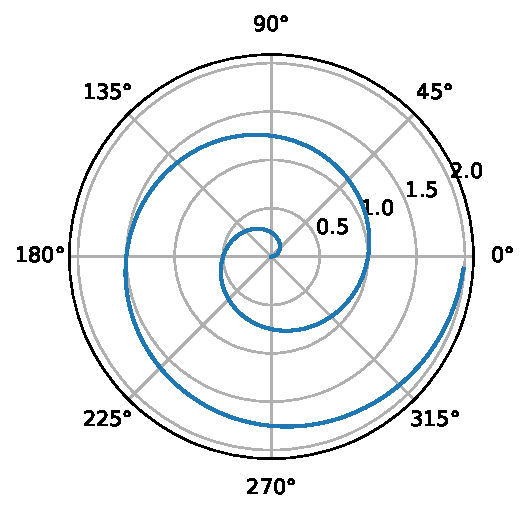
\includegraphics{./hello_files/figure-pdf/fig-polar-output-1.pdf}

}

\caption{\label{fig-polar}A line plot on a polar axis}

\end{figure}

\bookmarksetup{startatroot}

\hypertarget{quarto-computations}{%
\chapter{Quarto Computations}\label{quarto-computations}}

\begin{Shaded}
\begin{Highlighting}[]
\ImportTok{import}\NormalTok{ numpy }\ImportTok{as}\NormalTok{ np}
\NormalTok{a }\OperatorTok{=}\NormalTok{ np.arange(}\DecValTok{15}\NormalTok{).reshape(}\DecValTok{3}\NormalTok{, }\DecValTok{5}\NormalTok{)}
\NormalTok{a}
\end{Highlighting}
\end{Shaded}

\begin{verbatim}
array([[ 0,  1,  2,  3,  4],
       [ 5,  6,  7,  8,  9],
       [10, 11, 12, 13, 14]])
\end{verbatim}

\hypertarget{matplotlib}{%
\section{Matplotlib}\label{matplotlib}}

\begin{Shaded}
\begin{Highlighting}[]
\ImportTok{import}\NormalTok{ matplotlib.pyplot }\ImportTok{as}\NormalTok{ plt}

\NormalTok{fig }\OperatorTok{=}\NormalTok{ plt.figure()}
\NormalTok{x }\OperatorTok{=}\NormalTok{ np.arange(}\DecValTok{10}\NormalTok{)}
\NormalTok{y }\OperatorTok{=} \FloatTok{2.5} \OperatorTok{*}\NormalTok{ np.sin(x }\OperatorTok{/} \DecValTok{20} \OperatorTok{*}\NormalTok{ np.pi)}
\NormalTok{yerr }\OperatorTok{=}\NormalTok{ np.linspace(}\FloatTok{0.05}\NormalTok{, }\FloatTok{0.2}\NormalTok{, }\DecValTok{10}\NormalTok{)}

\NormalTok{plt.errorbar(x, y }\OperatorTok{+} \DecValTok{3}\NormalTok{, yerr}\OperatorTok{=}\NormalTok{yerr, label}\OperatorTok{=}\StringTok{\textquotesingle{}both limits (default)\textquotesingle{}}\NormalTok{)}
\NormalTok{plt.errorbar(x, y }\OperatorTok{+} \DecValTok{2}\NormalTok{, yerr}\OperatorTok{=}\NormalTok{yerr, uplims}\OperatorTok{=}\VariableTok{True}\NormalTok{, label}\OperatorTok{=}\StringTok{\textquotesingle{}uplims=True\textquotesingle{}}\NormalTok{)}
\NormalTok{plt.errorbar(x, y }\OperatorTok{+} \DecValTok{1}\NormalTok{, yerr}\OperatorTok{=}\NormalTok{yerr, uplims}\OperatorTok{=}\VariableTok{True}\NormalTok{, lolims}\OperatorTok{=}\VariableTok{True}\NormalTok{,}
\NormalTok{             label}\OperatorTok{=}\StringTok{\textquotesingle{}uplims=True, lolims=True\textquotesingle{}}\NormalTok{)}

\NormalTok{upperlimits }\OperatorTok{=}\NormalTok{ [}\VariableTok{True}\NormalTok{, }\VariableTok{False}\NormalTok{] }\OperatorTok{*} \DecValTok{5}
\NormalTok{lowerlimits }\OperatorTok{=}\NormalTok{ [}\VariableTok{False}\NormalTok{, }\VariableTok{True}\NormalTok{] }\OperatorTok{*} \DecValTok{5}
\NormalTok{plt.errorbar(x, y, yerr}\OperatorTok{=}\NormalTok{yerr, uplims}\OperatorTok{=}\NormalTok{upperlimits, lolims}\OperatorTok{=}\NormalTok{lowerlimits,}
\NormalTok{             label}\OperatorTok{=}\StringTok{\textquotesingle{}subsets of uplims and lolims\textquotesingle{}}\NormalTok{)}

\NormalTok{plt.legend(loc}\OperatorTok{=}\StringTok{\textquotesingle{}lower right\textquotesingle{}}\NormalTok{)}
\NormalTok{plt.show(fig)}
\end{Highlighting}
\end{Shaded}

\begin{figure}[H]

{\centering 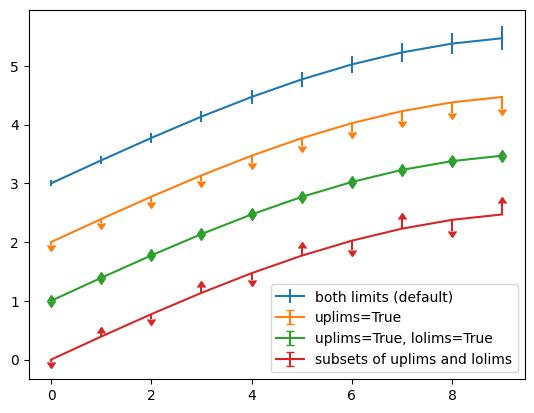
\includegraphics{./computations_files/figure-pdf/cell-3-output-1.png}

}

\end{figure}

\hypertarget{plotly}{%
\section{Plotly}\label{plotly}}

\begin{Shaded}
\begin{Highlighting}[]
\ImportTok{import}\NormalTok{ plotly.express }\ImportTok{as}\NormalTok{ px}
\ImportTok{import}\NormalTok{ plotly.io }\ImportTok{as}\NormalTok{ pio}
\NormalTok{gapminder }\OperatorTok{=}\NormalTok{ px.data.gapminder()}
\NormalTok{gapminder2007 }\OperatorTok{=}\NormalTok{ gapminder.query(}\StringTok{"year == 2007"}\NormalTok{)}
\NormalTok{fig }\OperatorTok{=}\NormalTok{ px.scatter(gapminder2007, }
\NormalTok{                 x}\OperatorTok{=}\StringTok{"gdpPercap"}\NormalTok{, y}\OperatorTok{=}\StringTok{"lifeExp"}\NormalTok{, color}\OperatorTok{=}\StringTok{"continent"}\NormalTok{, }
\NormalTok{                 size}\OperatorTok{=}\StringTok{"pop"}\NormalTok{, size\_max}\OperatorTok{=}\DecValTok{60}\NormalTok{,}
\NormalTok{                 hover\_name}\OperatorTok{=}\StringTok{"country"}\NormalTok{)}
\NormalTok{fig.show()}
\end{Highlighting}
\end{Shaded}

\begin{verbatim}
Unable to display output for mime type(s): application/vnd.plotly.v1+json
\end{verbatim}

\bookmarksetup{startatroot}

\hypertarget{image-from-linked-open-data-api}{%
\chapter{Image from linked open data
API}\label{image-from-linked-open-data-api}}

\hypertarget{image---siege-iii-the-fortress-of-raab-occupied-by-the-turks-1594.-painting-httpswikibase.wbworkshop.tibwiki.iowikiitemq505}{%
\subsection{Image - Siege III: The Fortress of Raab occupied by the
Turks, 1594. Painting,
https://wikibase.wbworkshop.tibwiki.io/wiki/Item:Q505}\label{image---siege-iii-the-fortress-of-raab-occupied-by-the-turks-1594.-painting-httpswikibase.wbworkshop.tibwiki.iowikiitemq505}}

The below Python code experiments with retrieving data from Wikibase
using the API. This takes approx. 18 seconds to run due to the size of
the images.

\begin{Shaded}
\begin{Highlighting}[]
\ImportTok{from}\NormalTok{ PIL }\ImportTok{import}\NormalTok{ Image}
\ImportTok{import}\NormalTok{ requests}

\CommentTok{\# Global variables}
\NormalTok{endpoint\_url }\OperatorTok{=} \StringTok{\textquotesingle{}https://wikibase.wbworkshop.tibwiki.io\textquotesingle{}}
\NormalTok{resource\_url }\OperatorTok{=} \StringTok{\textquotesingle{}/w/api.php\textquotesingle{}}
\NormalTok{entity\_id }\OperatorTok{=} \StringTok{\textquotesingle{}Q505\textquotesingle{}}

\KeywordTok{def}\NormalTok{ get\_entity (entity\_id):}
\NormalTok{    resourceUrl }\OperatorTok{=} \StringTok{\textquotesingle{}/w/api.php?action=wbgetentities\&format=json\&ids=\textquotesingle{}}\OperatorTok{+}\NormalTok{entity\_id}
\NormalTok{    uri }\OperatorTok{=}\NormalTok{ endpoint\_url }\OperatorTok{+}\NormalTok{ resourceUrl}
\NormalTok{    r }\OperatorTok{=}\NormalTok{ requests.get(uri)}
\NormalTok{    data }\OperatorTok{=}\NormalTok{ r.json()}
    \ControlFlowTok{return}\NormalTok{ data}

\NormalTok{media\_data }\OperatorTok{=}\NormalTok{ get\_entity(entity\_id)}
\NormalTok{claims }\OperatorTok{=}\NormalTok{ media\_data[}\StringTok{\textquotesingle{}entities\textquotesingle{}}\NormalTok{][entity\_id][}\StringTok{\textquotesingle{}claims\textquotesingle{}}\NormalTok{]}
\ControlFlowTok{for} \BuiltInTok{property}\NormalTok{, values }\KeywordTok{in}\NormalTok{ claims.items():}
    \ControlFlowTok{if} \BuiltInTok{property} \OperatorTok{==} \StringTok{\textquotesingle{}P22\textquotesingle{}}\NormalTok{:}
        \ControlFlowTok{for}\NormalTok{ value }\KeywordTok{in}\NormalTok{ values:}
\NormalTok{            image\_url }\OperatorTok{=}\NormalTok{ value[}\StringTok{\textquotesingle{}mainsnak\textquotesingle{}}\NormalTok{][}\StringTok{\textquotesingle{}datavalue\textquotesingle{}}\NormalTok{][}\StringTok{\textquotesingle{}value\textquotesingle{}}\NormalTok{]}
\NormalTok{            im }\OperatorTok{=}\NormalTok{ Image.}\BuiltInTok{open}\NormalTok{(requests.get(image\_url, stream}\OperatorTok{=}\VariableTok{True}\NormalTok{).raw)}
    \ControlFlowTok{elif} \BuiltInTok{property} \OperatorTok{==} \StringTok{\textquotesingle{}P23\textquotesingle{}}\NormalTok{:}
        \ControlFlowTok{for}\NormalTok{ value }\KeywordTok{in}\NormalTok{ values:}
\NormalTok{            entity\_id }\OperatorTok{=}\NormalTok{ value[}\StringTok{\textquotesingle{}mainsnak\textquotesingle{}}\NormalTok{][}\StringTok{\textquotesingle{}datavalue\textquotesingle{}}\NormalTok{][}\StringTok{\textquotesingle{}value\textquotesingle{}}\NormalTok{][}\StringTok{\textquotesingle{}id\textquotesingle{}}\NormalTok{]}
\NormalTok{            object\_data }\OperatorTok{=}\NormalTok{ get\_entity(entity\_id)}
\BuiltInTok{print}\NormalTok{(}\StringTok{\textquotesingle{}English title: \textquotesingle{}}\NormalTok{, object\_data[}\StringTok{\textquotesingle{}entities\textquotesingle{}}\NormalTok{][entity\_id][}\StringTok{\textquotesingle{}labels\textquotesingle{}}\NormalTok{][}\StringTok{\textquotesingle{}en\textquotesingle{}}\NormalTok{][}\StringTok{\textquotesingle{}value\textquotesingle{}}\NormalTok{])}
\NormalTok{display(im)}
\end{Highlighting}
\end{Shaded}

\begin{verbatim}
English title:  Siege III: The Fortress of Raab occupied by the Turks, 1594
\end{verbatim}

\begin{figure}[H]

{\centering \includegraphics{./lod_image_files/figure-pdf/cell-2-output-2.png}

}

\end{figure}

\bookmarksetup{startatroot}

\hypertarget{linked-open-data-query-from-sparql}{%
\chapter{Linked open data query from
SPARQL}\label{linked-open-data-query-from-sparql}}

The below Python code experiments with using SPARQLWrapper to retrieve
data from NFDI4Culture's Wikibase based on a SPARQL query.

\begin{Shaded}
\begin{Highlighting}[]
\ImportTok{from}\NormalTok{ SPARQLWrapper }\ImportTok{import}\NormalTok{ SPARQLWrapper, JSON}
\ImportTok{from}\NormalTok{ PIL }\ImportTok{import}\NormalTok{ Image}
\ImportTok{from}\NormalTok{ ipypublish }\ImportTok{import}\NormalTok{ nb\_setup}
\ImportTok{import}\NormalTok{ numpy }\ImportTok{as}\NormalTok{ np}
\ImportTok{import}\NormalTok{ pandas}
\ImportTok{import}\NormalTok{ requests}
\ImportTok{import}\NormalTok{ sparql\_dataframe}

\KeywordTok{def}\NormalTok{ get\_delay(date):}
    \ControlFlowTok{try}\NormalTok{:}
\NormalTok{        date }\OperatorTok{=}\NormalTok{ datetime.datetime.strptime(date, }\StringTok{\textquotesingle{}\%a, }\SpecialCharTok{\%d}\StringTok{ \%b \%Y \%H:\%M:\%S GMT\textquotesingle{}}\NormalTok{)}
\NormalTok{        timeout }\OperatorTok{=} \BuiltInTok{int}\NormalTok{((date }\OperatorTok{{-}}\NormalTok{ datetime.datetime.now()).total\_seconds())}
    \ControlFlowTok{except} \PreprocessorTok{ValueError}\NormalTok{:}
\NormalTok{        timeout }\OperatorTok{=} \BuiltInTok{int}\NormalTok{(date)}
    \ControlFlowTok{return}\NormalTok{ timeout}

\KeywordTok{def}\NormalTok{ get\_image(url, headers):}
\NormalTok{    r }\OperatorTok{=}\NormalTok{ requests.get(url, headers}\OperatorTok{=}\NormalTok{headers, stream}\OperatorTok{=}\VariableTok{True}\NormalTok{)}
    \ControlFlowTok{if}\NormalTok{ r.status\_code }\OperatorTok{==} \DecValTok{200}\NormalTok{:}
\NormalTok{        im }\OperatorTok{=}\NormalTok{ Image.}\BuiltInTok{open}\NormalTok{(r.raw)}
        \ControlFlowTok{return}\NormalTok{ im}
    \ControlFlowTok{if}\NormalTok{ r.status\_code }\OperatorTok{==} \DecValTok{500}\NormalTok{:}
        \ControlFlowTok{return} \VariableTok{None}
    \ControlFlowTok{if}\NormalTok{ r.status\_code }\OperatorTok{==} \DecValTok{403}\NormalTok{:}
        \ControlFlowTok{return} \VariableTok{None}
    \ControlFlowTok{if}\NormalTok{ r.status\_code }\OperatorTok{==} \DecValTok{429}\NormalTok{:}
\NormalTok{        timeout }\OperatorTok{=}\NormalTok{ get\_delay(r.headers[}\StringTok{\textquotesingle{}retry{-}after\textquotesingle{}}\NormalTok{])}
        \BuiltInTok{print}\NormalTok{(}\StringTok{\textquotesingle{}Timeout }\SpecialCharTok{\{\}}\StringTok{ m }\SpecialCharTok{\{\}}\StringTok{ s\textquotesingle{}}\NormalTok{.}\BuiltInTok{format}\NormalTok{(timeout }\OperatorTok{//} \DecValTok{60}\NormalTok{, timeout }\OperatorTok{\%} \DecValTok{60}\NormalTok{))}
\NormalTok{        time.sleep(timeout)}
\NormalTok{        get\_image(url, headers)}

\CommentTok{\# Example using NFDI4Culture Wikibase}

\CommentTok{\# Specify the NFDI4Culture Wikibase SPARQL endpoint}
\NormalTok{endpoint\_url }\OperatorTok{=} \StringTok{\textquotesingle{}https://query.wbworkshop.tibwiki.io/proxy/wdqs/bigdata/namespace/wdq/sparql\textquotesingle{}}

\CommentTok{\# Query}
\NormalTok{query }\OperatorTok{=} \StringTok{"""}
\StringTok{SELECT ?item ?itemLabel ?creationDateStart ?creationDateEnd ?inscription ?materialLabel ?methodLabel ?description ?media}
\StringTok{WHERE \{ }
\StringTok{    ?item tibt:P25 tib:Q60.}
\StringTok{    ?item tibt:P79 ?creationDateStart.}
\StringTok{    ?item tibt:P80 ?creationDateEnd.}
\StringTok{    ?item tibt:P18 ?inscription.}
\StringTok{    ?item tibt:P38 ?material.}
\StringTok{    ?item tibt:P39 ?method.}
\StringTok{    ?item tibt:P26 ?description.}
\StringTok{    ?item tibt:P16 ?media}
\StringTok{    SERVICE wikibase:label \{ bd:serviceParam wikibase:language "[AUTO\_LANGUAGE],en". \}}
\StringTok{\} }
\StringTok{\#All paintings from "Belagerungsszenen des Langen Türkenkriegs"}
\StringTok{"""}

\NormalTok{dataframe }\OperatorTok{=}\NormalTok{ sparql\_dataframe.get(endpoint\_url, query, post}\OperatorTok{=}\VariableTok{True}\NormalTok{)}

\NormalTok{dataframe}

\CommentTok{\# Example using Wikidata}

\CommentTok{\# Specify the Wikidata SPARQL endpoint}
\CommentTok{\#endpoint\_url = \textquotesingle{}https://query.wikidata.org/bigdata/namespace/wdq/sparql\textquotesingle{}}

\CommentTok{\#user\_agent = \textquotesingle{}cp4c\_bot/0.0 (https://github.com/SimonXIX/cp4c; ad7588@coventry.ac.uk)\textquotesingle{}}
\CommentTok{\#sparql = SPARQLWrapper(endpoint\_url, agent=user\_agent)}

\CommentTok{\# query = """}
\CommentTok{\# \#Cats, with pictures}
\CommentTok{\# \#defaultView:ImageGrid}
\CommentTok{\# SELECT ?item ?itemLabel ?pic}
\CommentTok{\# WHERE}
\CommentTok{\# \{}
\CommentTok{\# ?item wdt:P31 wd:Q146 .}
\CommentTok{\# ?item wdt:P18 ?pic}
\CommentTok{\# SERVICE wikibase:label \{ bd:serviceParam wikibase:language "[AUTO\_LANGUAGE],en" \}}
\CommentTok{\# \}}
\CommentTok{\# LIMIT 2}
\CommentTok{\# """}

\CommentTok{\# Retrieve results and convert to JSON format}
\CommentTok{\#sparql.setQuery(query)}
\CommentTok{\#sparql.setReturnFormat(JSON)}
\CommentTok{\#result = sparql.query().convert()}

\CommentTok{\#for item in result[\textquotesingle{}results\textquotesingle{}][\textquotesingle{}bindings\textquotesingle{}]:}
    \CommentTok{\# image\_url=item[\textquotesingle{}pic\textquotesingle{}][\textquotesingle{}value\textquotesingle{}]}
    \CommentTok{\# headers = \{\textquotesingle{}User{-}Agent\textquotesingle{}: \textquotesingle{}cp4c\_bot/0.0 (https://github.com/SimonXIX/cp4c; ad7588@coventry.ac.uk)\textquotesingle{}\}}
    \CommentTok{\# im = get\_image(image\_url, headers)}

    \CommentTok{\# print(\textquotesingle{}Cat name: \textquotesingle{}, item[\textquotesingle{}itemLabel\textquotesingle{}][\textquotesingle{}value\textquotesingle{}])}
    \CommentTok{\# display(im)}
\end{Highlighting}
\end{Shaded}

\begin{longtable}[]{@{}llllllllll@{}}
\toprule()
& item & itemLabel & creationDateStart & creationDateEnd & inscription &
materialLabel & methodLabel & description & media \\
\midrule()
\endhead
0 & https://wikibase.wbworkshop.tibwiki.io/entity/... & Siege VII: The
city of Waitzen occupied by the... & 1602-01-01T00:00:00Z &
1604-01-01T00:00:00Z & „Statt Waitzen wie die von vom Türcken beleger...
& Canvas & Oil painting &
https://wikibase.wbworkshop.tibwiki.io/entity/... &
https://wikibase.wbworkshop.tibwiki.io/entity/... \\
1 & https://wikibase.wbworkshop.tibwiki.io/entity/... & Siege I: The
Fortress of Tottis retaken by the... & 1602-01-01T00:00:00Z &
1604-01-01T00:00:00Z & „Vestung Tottis, wie die von den Christen bei ...
& Canvas & Oil painting &
https://wikibase.wbworkshop.tibwiki.io/entity/... &
https://wikibase.wbworkshop.tibwiki.io/entity/... \\
2 & https://wikibase.wbworkshop.tibwiki.io/entity/... & Siege II: The
Fortress of Gran occupied by the... & 1602-01-01T00:00:00Z &
1604-01-01T00:00:00Z & „Vestung Gran wie die von Christen belegert ge...
& Canvas & Oil painting &
https://wikibase.wbworkshop.tibwiki.io/entity/... &
https://wikibase.wbworkshop.tibwiki.io/entity/... \\
3 & https://wikibase.wbworkshop.tibwiki.io/entity/... & Siege XII: The
Fortress of Gran occupied by th... & 1602-01-01T00:00:00Z &
1604-01-01T00:00:00Z & „Vestung Gran wie die vom Türcken belegert gew...
& Canvas & Oil painting &
https://wikibase.wbworkshop.tibwiki.io/entity/... &
https://wikibase.wbworkshop.tibwiki.io/entity/... \\
4 & https://wikibase.wbworkshop.tibwiki.io/entity/... & Siege XI: The
capital city Offen occupied by t... & 1602-01-01T00:00:00Z &
1604-01-01T00:00:00Z & „Hauptstatt Offen, wie die von Christn beleger...
& Canvas & Oil painting &
https://wikibase.wbworkshop.tibwiki.io/entity/... &
https://wikibase.wbworkshop.tibwiki.io/entity/... \\
5 & https://wikibase.wbworkshop.tibwiki.io/entity/... & Siege III: The
Fortress of Raab occupied by th... & 1602-01-01T00:00:00Z &
1604-01-01T00:00:00Z & „Vestung Raab, wie die vom Türcken belegert ge...
& Canvas & Oil painting &
https://wikibase.wbworkshop.tibwiki.io/entity/... &
https://wikibase.wbworkshop.tibwiki.io/entity/... \\
6 & https://wikibase.wbworkshop.tibwiki.io/entity/... & Siege IV: The
Fortress of Comorna occupied by ... & 1602-01-01T00:00:00Z &
1604-01-01T00:00:00Z & „Vestung Comorna wie die vom Türckn belegert g...
& Canvas & Oil painting &
https://wikibase.wbworkshop.tibwiki.io/entity/... &
https://wikibase.wbworkshop.tibwiki.io/entity/... \\
7 & https://wikibase.wbworkshop.tibwiki.io/entity/... & Siege V: The
Fortress of Gran retaken by the C... & 1602-01-01T00:00:00Z &
1604-01-01T00:00:00Z & „Vestung Gran wie die von den Christen wider e...
& Canvas & Oil painting &
https://wikibase.wbworkshop.tibwiki.io/entity/... &
https://wikibase.wbworkshop.tibwiki.io/entity/... \\
8 & https://wikibase.wbworkshop.tibwiki.io/entity/... & Siege VI: The
Fortress of Vizzegrad occupied b... & 1602-01-01T00:00:00Z &
1604-01-01T00:00:00Z & ``Vestung Vizzegrad wie die von Christen
belege... & Canvas & Oil painting &
https://wikibase.wbworkshop.tibwiki.io/entity/... &
https://wikibase.wbworkshop.tibwiki.io/entity/... \\
9 & https://wikibase.wbworkshop.tibwiki.io/entity/... & Siege VIII: The
Fortress of Raab, which was re... & 1602-01-01T00:00:00Z &
1604-01-01T00:00:00Z & „Vestung Raab, die Christen beÿ der Nacht wide...
& Canvas & Oil painting &
https://wikibase.wbworkshop.tibwiki.io/entity/... &
https://wikibase.wbworkshop.tibwiki.io/entity/... \\
10 & https://wikibase.wbworkshop.tibwiki.io/entity/... & Siege IX: The
capital city Offen occupied by t... & 1602-01-01T00:00:00Z &
1604-01-01T00:00:00Z & „Hauptstatt Offen. wie die von Christen belege...
& Canvas & Oil painting &
https://wikibase.wbworkshop.tibwiki.io/entity/... &
https://wikibase.wbworkshop.tibwiki.io/entity/... \\
11 & https://wikibase.wbworkshop.tibwiki.io/entity/... & Siege X: The
capital city Offen occupied by th... & 1602-01-01T00:00:00Z &
1604-01-01T00:00:00Z & „Hauptstatt Offen, wie die von Christen belege...
& Canvas & Oil painting &
https://wikibase.wbworkshop.tibwiki.io/entity/... &
https://wikibase.wbworkshop.tibwiki.io/entity/... \\
\bottomrule()
\end{longtable}

\bookmarksetup{startatroot}

\hypertarget{d-model-with-annotations}{%
\chapter{3D model with annotations}\label{d-model-with-annotations}}

\bookmarksetup{startatroot}

\hypertarget{embedded-video}{%
\chapter{Embedded video}\label{embedded-video}}

The below Python code experiments with retrieving video data via iframe
embedding.

\begin{Shaded}
\begin{Highlighting}[]
\ImportTok{from}\NormalTok{ IPython.display }\ImportTok{import}\NormalTok{ HTML}
\NormalTok{HTML(}\StringTok{"""}
\StringTok{\textless{}iframe width="560" height="315" scrolling="no" src="https://av.tib.eu/player/56162" frameborder="0" allowfullscreen\textgreater{}\textless{}/iframe\textgreater{}}
\StringTok{"""}\NormalTok{)}
\end{Highlighting}
\end{Shaded}

\begin{verbatim}
<IPython.core.display.HTML object>
\end{verbatim}

\bookmarksetup{startatroot}

\hypertarget{linked-open-data-api-testing}{%
\chapter{Linked open data API
testing}\label{linked-open-data-api-testing}}

This notebook experiments with querying linked open data in a Jupyter
Notebook rendered through Quarto.

The Python code below queries the NFDI4Culture Wikibase at
https://wikibase.wbworkshop.tibwiki.io/wiki/Main\_Page and returns data
based on the ID inputted by the user.

This executes in Jupyter Notebook which is able to run the Python code
and provides a static output when saved in the Notebook. It cannot be
executed dynamically in Quarto since the Quarto front-end does not
support stdin input requests.

To reset the output, run `Kernel \textgreater{} Restart kernel and clear
all outputs'.

\hypertarget{wikibase-api-testing}{%
\section{Wikibase API testing}\label{wikibase-api-testing}}

\begin{Shaded}
\begin{Highlighting}[]
\ImportTok{import}\NormalTok{ requests}

\CommentTok{\# Global variables}
\NormalTok{endpoint\_url }\OperatorTok{=} \StringTok{\textquotesingle{}https://wikibase.wbworkshop.tibwiki.io\textquotesingle{}}
\NormalTok{resource\_url }\OperatorTok{=} \StringTok{\textquotesingle{}/w/api.php\textquotesingle{}}

\NormalTok{entity }\OperatorTok{=} \BuiltInTok{input}\NormalTok{(}\StringTok{"What\textquotesingle{}s the Q number (including the \textquotesingle{}Q\textquotesingle{})? "}\NormalTok{)}
\BuiltInTok{print}\NormalTok{(}\StringTok{\textquotesingle{}Check out \textquotesingle{}} \OperatorTok{+}\NormalTok{ endpoint\_url }\OperatorTok{+} \StringTok{\textquotesingle{}/wiki/\textquotesingle{}} \OperatorTok{+}\NormalTok{ entity }\OperatorTok{+} \StringTok{\textquotesingle{} to see the GUI.\textquotesingle{}}\NormalTok{)}
\NormalTok{resourceUrl }\OperatorTok{=} \StringTok{\textquotesingle{}/w/api.php?action=wbgetclaims\&format=json\&entity=\textquotesingle{}}\OperatorTok{+}\NormalTok{entity}
\NormalTok{uri }\OperatorTok{=}\NormalTok{ endpoint\_url }\OperatorTok{+}\NormalTok{ resourceUrl}
\NormalTok{r }\OperatorTok{=}\NormalTok{ requests.get(uri)}
\NormalTok{data }\OperatorTok{=}\NormalTok{ r.json()}
\NormalTok{claims }\OperatorTok{=}\NormalTok{ data[}\StringTok{\textquotesingle{}claims\textquotesingle{}}\NormalTok{]}
\BuiltInTok{print}\NormalTok{(}\StringTok{\textquotesingle{}subject: \textquotesingle{}}\NormalTok{, entity)}
\BuiltInTok{print}\NormalTok{()}
\ControlFlowTok{for} \BuiltInTok{property}\NormalTok{, values }\KeywordTok{in}\NormalTok{ claims.items():}
    \BuiltInTok{print}\NormalTok{(}\StringTok{\textquotesingle{}property: \textquotesingle{}}\NormalTok{, }\BuiltInTok{property}\NormalTok{)}
    \ControlFlowTok{for}\NormalTok{ value }\KeywordTok{in}\NormalTok{ values:}
        \ControlFlowTok{try}\NormalTok{:}
            \CommentTok{\# print Q ID if the value is an item}
            \BuiltInTok{print}\NormalTok{(}\StringTok{\textquotesingle{}item value: \textquotesingle{}}\NormalTok{, value[}\StringTok{\textquotesingle{}mainsnak\textquotesingle{}}\NormalTok{][}\StringTok{\textquotesingle{}datavalue\textquotesingle{}}\NormalTok{][}\StringTok{\textquotesingle{}value\textquotesingle{}}\NormalTok{][}\StringTok{\textquotesingle{}id\textquotesingle{}}\NormalTok{])}
        \ControlFlowTok{except}\NormalTok{:}
            \ControlFlowTok{try}\NormalTok{:}
                \CommentTok{\# print the string value if the value is a literal}
                \BuiltInTok{print}\NormalTok{(}\StringTok{\textquotesingle{}literal value: \textquotesingle{}}\NormalTok{, value[}\StringTok{\textquotesingle{}mainsnak\textquotesingle{}}\NormalTok{][}\StringTok{\textquotesingle{}datavalue\textquotesingle{}}\NormalTok{][}\StringTok{\textquotesingle{}value\textquotesingle{}}\NormalTok{])}
            \ControlFlowTok{except}\NormalTok{:}
                \CommentTok{\# print the whole snak if the value is something else}
                \BuiltInTok{print}\NormalTok{(}\StringTok{\textquotesingle{}other value: \textquotesingle{}}\NormalTok{, value[}\StringTok{\textquotesingle{}mainsnak\textquotesingle{}}\NormalTok{])}
    \BuiltInTok{print}\NormalTok{()}
\end{Highlighting}
\end{Shaded}

\bookmarksetup{startatroot}

\hypertarget{query-orcid-for-works-authored-by-a-person}{%
\chapter{Query ORCID for works authored by a
person}\label{query-orcid-for-works-authored-by-a-person}}

Taken from Project TAPIR's repository of Jupyter Notebooks:
https://github.com/Project-TAPIR/pidgraph-notebooks

This notebook queries the \href{https://pub.orcid.org/v3.0/}{ORCID
Public API} to retrieve works listed in a person's ORCID record. It
takes an ORCID URL or iD as input to retrieve the ORCID record of a
person and the works listed on it. From the resulting list of works we
output all DOIs.

\begin{Shaded}
\begin{Highlighting}[]
\CommentTok{\# Prerequisites:}
\ImportTok{import}\NormalTok{ requests                        }\CommentTok{\# dependency to make HTTP calls}
\ImportTok{from}\NormalTok{ benedict }\ImportTok{import}\NormalTok{ benedict          }\CommentTok{\# dependency for dealing with json}
\end{Highlighting}
\end{Shaded}

The input for this notebook is an ORCID URL or iD,
e.g.~`\texttt{https://orcid.org/0000-0003-2499-7741}' or
`\texttt{0000-0003-2499-7741}'.

\begin{Shaded}
\begin{Highlighting}[]
\CommentTok{\# input parameter}
\NormalTok{example\_orcid}\OperatorTok{=}\StringTok{"https://orcid.org/0000{-}0002{-}2437{-}589X"}
\end{Highlighting}
\end{Shaded}

We use it to query ORCID's Public API for the person's metadata and all
works connected to them.

\begin{Shaded}
\begin{Highlighting}[]
\CommentTok{\# URL for ORCID API}
\NormalTok{ORCID\_RECORD\_API }\OperatorTok{=} \StringTok{"https://pub.orcid.org/v3.0/"}

\CommentTok{\# query ORCID for an ORCID record}
\KeywordTok{def}\NormalTok{ query\_orcid\_for\_record(orcid\_id):}

\NormalTok{    response }\OperatorTok{=}\NormalTok{ requests.get(url}\OperatorTok{=}\NormalTok{requests.utils.requote\_uri(ORCID\_RECORD\_API }\OperatorTok{+}\NormalTok{ orcid\_id),}
\NormalTok{                          headers}\OperatorTok{=}\NormalTok{\{}\StringTok{\textquotesingle{}Accept\textquotesingle{}}\NormalTok{: }\StringTok{\textquotesingle{}application/json\textquotesingle{}}\NormalTok{\})}
\NormalTok{    response.raise\_for\_status()}
\NormalTok{    result}\OperatorTok{=}\NormalTok{response.json()}
    \ControlFlowTok{return}\NormalTok{ result}


\CommentTok{\#{-}{-} example execution}
\NormalTok{orcid\_id}\OperatorTok{=}\NormalTok{example\_orcid.replace(}\StringTok{"https://orcid.org/"}\NormalTok{, }\StringTok{""}\NormalTok{)}
\NormalTok{orcid\_record}\OperatorTok{=}\NormalTok{query\_orcid\_for\_record(orcid\_id)}
\CommentTok{\# uncomment next lines to see complete metadata for given ORCID}
\CommentTok{\#import pprint}
\CommentTok{\#pprint.pprint(orcid\_record)}
\end{Highlighting}
\end{Shaded}

From the complete ORCID metadata we extract the works section and print
out title and DOI of each first \texttt{work-summary} (the first item in
a personal information section has the highest
\href{https://info.orcid.org/documentation/integration-guide/orcid-record/\#Display_index}{display
index}).

\emph{Note: works that do not have a DOI assigned, will not be printed.}

\begin{Shaded}
\begin{Highlighting}[]
\CommentTok{\# extract works section from ORCID profile}
\KeywordTok{def}\NormalTok{ extract\_works\_section(orcid\_record):}
\NormalTok{    orcid\_dict}\OperatorTok{=}\NormalTok{benedict.from\_json(orcid\_record)}
\NormalTok{    works}\OperatorTok{=}\NormalTok{orcid\_dict.get(}\StringTok{\textquotesingle{}activities{-}summary.works.group\textquotesingle{}}\NormalTok{) }\KeywordTok{or}\NormalTok{ []}
    \ControlFlowTok{return}\NormalTok{ works}

\CommentTok{\# for each work in the work section: extract title and DOI}
\KeywordTok{def}\NormalTok{ extract\_doi(work):}
\NormalTok{    work\_dict}\OperatorTok{=}\NormalTok{benedict.from\_json(work)}
\NormalTok{    title}\OperatorTok{=}\NormalTok{work\_dict.get(}\StringTok{\textquotesingle{}work{-}summary[0].title.title.value\textquotesingle{}}\NormalTok{)}
\NormalTok{    dois}\OperatorTok{=}\NormalTok{ [doi[}\StringTok{\textquotesingle{}external{-}id{-}value\textquotesingle{}}\NormalTok{] }\ControlFlowTok{for}\NormalTok{ doi }\KeywordTok{in}\NormalTok{ work\_dict.get(}\StringTok{\textquotesingle{}work{-}summary[0].external{-}ids.external{-}id\textquotesingle{}}\NormalTok{, []) }\ControlFlowTok{if}\NormalTok{ doi[}\StringTok{\textquotesingle{}external{-}id{-}type\textquotesingle{}}\NormalTok{]}\OperatorTok{==}\StringTok{"doi"}\NormalTok{]}
    \CommentTok{\# if there is a DOI assigned to the work, the list of dois is not empty and we can extract the first one}
\NormalTok{    doi}\OperatorTok{=}\NormalTok{dois[}\DecValTok{0}\NormalTok{] }\ControlFlowTok{if}\NormalTok{ dois }\ControlFlowTok{else} \VariableTok{None}
    \ControlFlowTok{return}\NormalTok{ doi, title}


\CommentTok{\# {-}{-}{-}{-} example execution}
\NormalTok{works}\OperatorTok{=}\NormalTok{extract\_works\_section(orcid\_record)}
\ControlFlowTok{for}\NormalTok{ work }\KeywordTok{in}\NormalTok{ works:}
\NormalTok{    doi,title }\OperatorTok{=}\NormalTok{ extract\_doi(work)}
    \ControlFlowTok{if}\NormalTok{ doi:}
        \BuiltInTok{print}\NormalTok{(}\SpecialStringTok{f"}\SpecialCharTok{\{}\NormalTok{doi}\SpecialCharTok{\}}\SpecialStringTok{, }\SpecialCharTok{\{}\NormalTok{title}\SpecialCharTok{\}}\SpecialStringTok{"}\NormalTok{)}
\end{Highlighting}
\end{Shaded}

\begin{verbatim}
10.21428/785a6451.af466093, What is computational publishing?
10.21428/785a6451.1792b84f, Books Contain Multitudes
10.21428/785a6451.0ed93b68, Part 1: Mapping & Situating Experimental Books
10.21428/785a6451.cd58a48e, Part 2: A Typology of Experimental Books
10.21428/785a6451.c4d3ffa1, Introducing COPIM's new website
10.17613/d4rs-rx03, Posthumanism in Outer Wilds
10.17613/5SJE-W447, New Sincerity, the Weird, and the post-ironic turn in contemporary indie video games
10.20944/preprints202001.0240.v1, Open or Ajar? Openness within the Neoliberal Academy
\end{verbatim}

\bookmarksetup{startatroot}

\hypertarget{references}{%
\chapter*{References}\label{references}}
\addcontentsline{toc}{chapter}{References}

\markboth{References}{References}

\hypertarget{refs}{}
\begin{CSLReferences}{1}{0}
\leavevmode\vadjust pre{\hypertarget{ref-knuth84}{}}%
Knuth, Donald E. 1984. {``Literate Programming.''} \emph{Comput. J.} 27
(2): 97--111. \url{https://doi.org/10.1093/comjnl/27.2.97}.

\end{CSLReferences}



\end{document}
